\section{Adjustments to GGR algorithm}

The pseudocode specification of Adjusted GGR can be found in Algorithm~\ref{alg:greedy-adj} listing.

\input{sections/2_1_ggr_alg_greedy_adj}

\vspace{-0.5em}

\subsection{Early Termination} %\label{sec:adj-early-exit}

\vspace{-0.5em}

\subsection{Faster Table Scan with FD and Table Statistics} %\label{sec:adj-table-stats}

\vspace{-0.5em}

\subsection{$K$ Top Hit Counts in One Column} %\label{sec:adj-k-top}

There could be a case when some column $A$ has a distinct value $a1$ with max
hit count, but then it has another distinct value $a2$ with the second-highest
hit count.
In general, the column might have $K$ distinct values with the top hit counts
(some of them can be ties).

This is a typical case for tables with a very low cardinality metadata column
that can easily contain distinct values with (almost) all top hit counts.
Consider an example of a ``Device Type'' column with three distinct values
``Android Device'', ``iOS Device'', and ``Web Browser'' -- all with the top hit counts.

Another example of this case is when most columns have zero hit count distinct
values, but one column has lots of distinct values with low but non-zero hit
counts.

We can exploit cases like this by splitting the table into $K+1$ sub-tables in
one iteration rather than going through $K$ separate iterations.
It also accelerates the reduction of sub-table size benefitting the table scan in
subsequent recursions.
See Figure~\ref{fig:2-01-aggr-k-top} for a description of this adjustment.

We can characterize this approach as an extension of the ``greedy'' strategy to
selecting multiple distinct values in one column in one iteration.

Note that this adjustment does not improve the output optimality but reduces the
number of iterations, in some cases significantly.

\begin{figure}
    \centering
    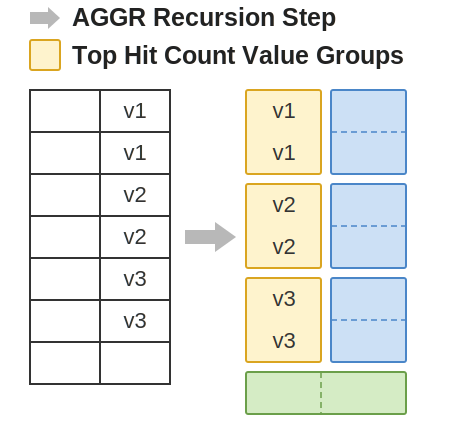
\includegraphics[width=0.49\textwidth]{figures/claude-figures/2-01-aggr-k-top}
    \vspace{-1.5em}
    \caption{
        If a column $V$ contains $K$ distinct values $v1, v2, \dots, vK$ with the highest
        hit counts in the table, Adjusted GGR picks all $K$ top hit count groups in
        one recursion step and splits the table into $K+1$ sub-tables: one sub-table
        $T$ excluding rows $\sum_{i=1}^{K} R_{vi}$ (green box), and $K$ sub-tables
        of rows $R_{vi}$ for $i \in 1 \dots K$ excluding the column $V$ (blue boxes).
    }
    \label{fig:2-01-aggr-k-top}
    \vspace{-1.5em}
\end{figure}

\vspace{-0.5em}

\subsection{Max Hit Count Ties Across Columns} %\label{sec:adj-ties}

\vspace{-0.5em}

\subsection{Multiple Columns with the same number of Max Hit Count Ties} %\label{sec:adj-ties-cols}

\vspace{-0.5em}

\subsection{Ad-hoc heuristics for correlated distinct values} %\label{sec:adj-early-exit}

